\beginsong{Endlos lang zieht sich die Straße}[
    wuw={turi (Kurt Kremers), Nerother Wandervogel}, 
    jahr={1962}, 
    bo={112}, 
    pfii={32},
    gruen={59},
    siru={69},
]

\beginverse
\endverse
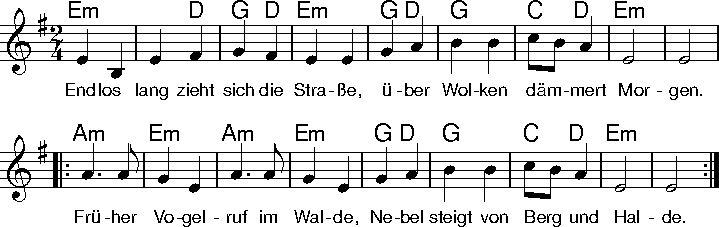
\includegraphics[draft=false, width=1\textwidth]{Noten/Lied034.pdf}	

\beginverse
\[Em]Auf dem blau\[D]en \[G]Tuch \[D]der \[Em]Blusen \[G]liegt \[D]der \[G]Staub der \[C]vie\[D]len \[Em]Stunden.
\lrep \[Am]Schweigend \[Em]zieht die \[Am]junge \[Em]Horde,
\[G]wei\[D]ter \[G]Weg braucht \[C]we\[D]nig \[Em]Worte. \rrep
\endverse

\beginverse
^Wer kann uns'^re ^We^ge ^messen? ^Wer ^kann ^unser ^Wol^len ^wägen?
\lrep ^Alle, ^die mit ^uns mar^schieren,
^wer^den ^Weg und ^Ziel ^er^spüren. \rrep
\endverse

\beginverse
^Neuer Tag ^wird ^Son^ne ^bringen; ^Son^ne ^ruft das ^jun^ge ^Leben.
\lrep ^Dunkel ^kann es ^nicht mehr ^halten,
^muss ^zu ^Hohem ^sich ^ent^falten. \rrep
\endverse

\endsong

\beginscripture{}
turi (*1920), zuvor Mitglied in einer dem Wandervogel ähnlichen Gruppierung, war im Dritten Reich unter Hitler verbotenerweise weiterhin mit anderen Bündischen auf Fahrt und hatte mehrmals Probleme mit der Gestapo, musste als Moorsaldat in Lagern schuften. Seiner reichskritischen Haltung entsprechend sind auch seine Lieder meist metaphorisch zu verstehen.
\endscripture
